\begin{figure}
    \centering
    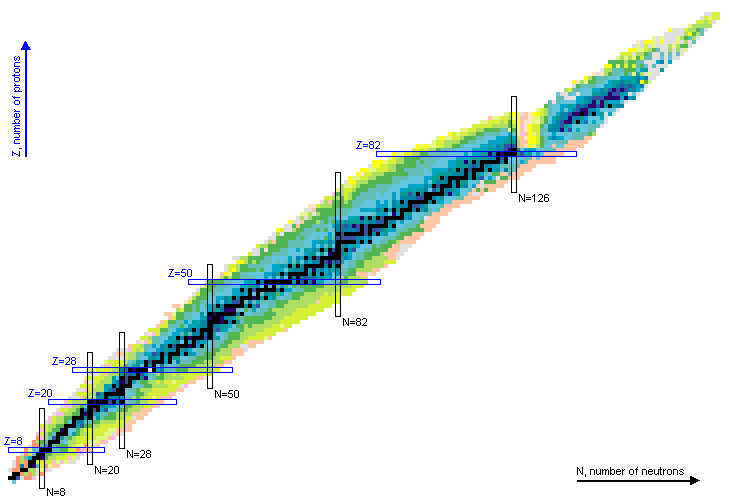
\includegraphics[scale=0.5]{Introduction_Figs/chartofnuclides_nndc.png}
    \caption{The chart of nuclides. The $x$-axis is increasing in neutron number from left to right, and the $y$-axis is increasing in proton number from bottom to top. The lower leftmost corner is the lightest elements, while the upper right are the heaviest, including superheavy elements. Black boxes indicate stable nuclei. These nuclei are in the "center" of the chart, and known colloquially as the valley of stability. To either side of these stable nuclei are radioactive nuclei, which become shorter lived the farther they are from the valley, indicated by the lightening color. The lines marked at 2, 8, 20 etc. are the closed shells for spherical nuclei, and are discussed in further depth within the text. Taken from \citep{nndc:_chart}.}
    \label{fig:chart}
\end{figure}